% A TikZ figure compiled on its own to a PDF cropped to the picture.
%   pdflatex -interaction=nonstopmode -halt-on-error figure.tex
% Needs only the tikz package: the page is sized to the picture with pdfTeX
% primitives, so the standalone and preview packages are not required.
\documentclass{article}
\usepackage[T1]{fontenc}
% Match the paper. Latin Modern Sans is in every TeX installation.
% With full TeX Live, \usepackage{helvet} gives Helvetica, and
% \usepackage{newtxtext,newtxmath} gives Times for IEEE-style serif text.
\usepackage{lmodern}
\renewcommand\familydefault{\sfdefault}
\usepackage{tikz}
\usetikzlibrary{positioning, arrows.meta, fit, calc, backgrounds}

% Style tokens for every figure of the paper. Keep them in one file
% (\input{figstyle}) when the paper has more than one TikZ figure.
\tikzset{
  every picture/.style={font=\footnotesize, line width=0.8pt, >={Stealth[length=2mm]}},
  block/.style={draw, minimum width=20mm, minimum height=7mm, align=center},
  group/.style={draw, inner sep=3mm, fill=black!4},
  emph/.style={fill=black!18},
  lbl/.style={font=\scriptsize, fill=white, inner sep=1pt},
  hair/.style={line width=0.4pt},
}

\begin{document}
\setbox0\hbox{%
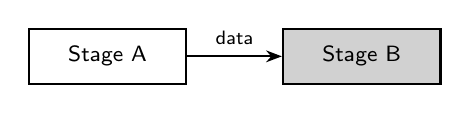
\begin{tikzpicture}
  \node[block] (a) {Stage A};
  \node[block, emph, right=12mm of a] (b) {Stage B};
  \draw[->] (a) -- node[lbl, above=1mm] {data} (b);
\end{tikzpicture}}%
\pdfpagewidth=\wd0 \pdfpageheight=\dimexpr\ht0+\dp0\relax
\hoffset=-1in \voffset=-1in
\shipout\box0
\end{document}
